% \documentclass[ba,preprint]{imsart}% use this for supplement article
\documentclass[ba]{imsart}
%
\pubyear{2022}
\volume{TBA}
\issue{TBA}
\doi{0000}
\arxiv{2010.00000}
\firstpage{1}
\lastpage{1}

%
\usepackage{amsthm}
\usepackage{amsmath}
\usepackage{amssymb}
\usepackage{natbib}
\usepackage[
  colorlinks,
  citecolor=blue,
  urlcolor=blue,
  filecolor=blue,
  backref=page
]{hyperref}
\usepackage{graphicx}

\startlocaldefs
\numberwithin{equation}{section}
\theoremstyle{plain}
\newtheorem{thm}{Theorem}[section]
\newtheorem{prop}{Proposition}[section]

\renewcommand{\epsilon}{\varepsilon}

\newcommand{\N}{\mathbb{N}}
\newcommand{\R}{\mathbb{R}}
\newcommand{\E}{\mathbb{E}}
\newcommand{\Var}{\ensuremath\operatorname{Var}}

%% Scalar product
\newcommand\dotprod[2]{\left\langle #1, #2 \right\rangle}

%% Environment for colored comments
\newenvironment{comment}
{
\noindent \em \color{red}
}
{
\color{black}
}

%% Inline comments
\newcommand\incomment[1]{\color{red}[\textit{#1}]\color{black}}
\endlocaldefs

\begin{document}

\begin{frontmatter}
\title{Bayesian RKHS-based methods in functional regression\support{Support information of the article.}}
\runtitle{Bayesian RKHS-based methods in functional regression }

\begin{aug}
\author{\fnms{First} \snm{Author}\thanksref{addr1,t1,t2,m1}\ead[label=e1]{first@somewhere.com}},
\author{\fnms{Second} \snm{Author}\thanksref{addr1,t3,m1,m2}\ead[label=e2]{second@somewhere.com}}
\and
\author{\fnms{Third} \snm{Author}\thanksref{addr2,t1,m2}%
\ead[label=e3]{third@somewhere.com}%
\ead[label=u1,url]{http://www.foo.com}}

\runauthor{F. Author et al.}

\address[addr1]{Address of the First and Second authors
     Usually a few lines long
    \printead{e1} % print email address of "e1"
    \printead*{e2}
}

\address[addr2]{Address of the Third author
    Usually a few lines long
    Usually a few lines long
    \printead{e3}
    \printead{u1}
}

\thankstext{t1}{Some comment}
\thankstext{t2}{First supporter of the project}
\thankstext{t3}{Second supporter of the project}

\end{aug}

\begin{abstract}
In this work we propose a Bayesian approach for functional linear or logistic  regression models, based on the theory of Reproducing Kernel Hilbert Spaces (RKHS's). These new models build upon the RKHS associated with the covariance function of the underlying stochastic process, and can be viewed as a finite-dimensional alternative to the classical functional regression paradigm. The corresponding functional model (or the functional logistic equation in the case of binary response) is determined by a function living on a dense subset of the RKHS generated by the underlying covariance function. By imposing a suitable prior distribution on such RKHS, we can perform data-driven inference via standard Bayes methodology. The posterior distribution can be approximated from Markov Chain Monte Carlo (MCMC) methods. Several estimators derived from this posterior distribution turn out to be competitive against other usual  alternatives in both simulated examples and real data sets, including a Bayesian-motivated variable selection method.
\end{abstract}

\begin{keyword}[class=MSC]
\kwd[Primary ]{62M20}
\kwd[; secondary ]{62F15}
\end{keyword}

\begin{keyword}
\kwd{functional data}
\kwd{linear regression}
\kwd{logistic regression}
\kwd{reproducing kernel Hilbert space}
\kwd{Bayesian inference}
\end{keyword}

\end{frontmatter}

\section{Introduction}\label{sec:intro}

The problem of inferring a scalar response from a functional covariate is one that has gained traction over the last few decades, as more and more data is being generated with an ever-increasing level of granularity in the measurements. While in principle we could simply treat the functional data as a discretized vector in a very high dimension, there are often many advantages in taking into account the functional nature of the data, ranging from modeling the possibly high correlation among points that are close in the domain, to extracting information that may be hidden in the derivatives of the function in question. As a consequence, numerous proposals have arisen on how to suitably treat functional data, all of them encompassed under the term Functional Data Analysis (FDA), which essentially explores statistical techniques to process, model and make inference on continuous data. A recent survey on such techniques and methods is \citet{cuevas2014partial}, while a more detailed exposition of the theory and applications can be found for example in \citet{hsing2015theoretical} and \citet{horváth2012inference}.

In this work we are concerned with (supervised) functional linear and logistic regression models, that is, situations where the goal is to predict a continuous or dichotomous variable from functional observations. Even though these problems can be formally stated with almost no differences from their finite-dimensional counterparts, there are some fundamental challenges that emerge as a result of working in infinite dimensions. To set a common framework, throughout this work we will consider a scalar response variable \(Y\) (either continuous or binary) which has some hidden dependence on a stochastic \(L^2\)-process \(X=X(t)=X(t, \omega)\) with trajectories in \(L^2[0, 1]\). We will assume the existence of a ``labeled'' data set \(\mathcal D_n =\{(X_i, Y_i): i=1,\dots, n\}\) of independent observations from \((X, Y)\), and our aim will be to accurately predict the response corresponding to unlabeled samples from \(X\).

The most common functional linear regression model is the classical \(L^2\)-model, originally introduced in the first edition of the book by~\citet{ramsay2005functional} \incomment{fue realmente así?}. It can be seen as a generalization of the usual finite-dimensional model, replacing the scalar product in \(\R^d\) for that of the functional space \(L^2[0,1]\):
\begin{equation}\label{eq:l2-linear-model}
Y = \beta_0 + \dotprod{X}{\beta} + \epsilon = \beta_0 + \int_0^1 X(t)\beta(t)\, dt + \epsilon,
\end{equation}
\incomment{mejor poner el producto con el subíndice \(\langle \cdot , \cdot \rangle_2\)?}~where \(\beta_0\in \R\) and \(\epsilon\) is an independent error term with certain simplifying assumptions. In this case, the main parameter \(\beta=\beta(t)\) is a member of the infinite-dimensional space \(L^2[0, 1]\). Aside from the fact that functional (i.e. infinite-dimensional) optimization is a hard problem in and of itself \incomment{cita?}, there are a number of more subtle drawbacks that arise in this \(L^2\)-framework. For instance, \(L^2[0, 1]\) is a big space that contains many non-smooth or ill-behaved functions, but incidentally the model given by~\eqref{eq:l2-linear-model} does not include a finite-dimensional model based on a linear combination of projections of \(X\) as a particular case \citep[see][]{berrendero2019rkhs}. Moreover, the non-invertibility of the covariance operator associated with \(X\) (defined in Section~\ref{sec:rkhs}), which plays the role of the covariance matrix in the infinite case, invalidates the usual least squares theory.

A similar \(L^2\)-based functional logistic equation can be derived for the binary classification problem via the logistic function:
\begin{equation}\label{eq:l2-logistic-model}
  \mathbb P(Y=1 \mid X) = \frac{1}{1 + \exp\{-\beta_0 - \dotprod{X}{\beta}\}},
\end{equation}
where \(\beta_0 \in \R\) and \(\beta \in L^2[0, 1]\). In this case, the most common way of estimating the slope function \(\beta(t)\) is via its Maximum Likelihood Estimator (MLE). However, not only do the same complications as in the linear regression model apply in this situation, but there is also the additional problem that in functional settings the MLE does not exist with probability one under fairly general conditions \citep[see][Sec.~3.2]{buenolarraz2021functional}.

It turns out that in both situations a natural alternative to the \(L^2\)-model is the so-called Reproducing Kernel Hilbert Space (RKHS) model, which instead assumes the unknown parameter to be a member of the RKHS associated with the covariance function of the process \(X\), making use of the scalar product of that space. As we will show later on, not only is this model simpler and arguably easier to interpret, but it also constrains the parameter space to smoother and more manageable functions. These RKHS-based models have already been explored in \citet{berrendero2020general} in the functional linear regression setting, and in \citet{berrendero2018use} for the case of functional classification. The main contribution of this work is a parametric Bayesian approach to parameter estimation within these recently-proposed models, in which a prior distribution is imposed on the unknown function to  obtain a posterior distribution after seeing the data.

Another set of techniques widely studied in this context are variable selection methods, which aim to select the marginals \(\{X(t_i)\}\) of the process that better summarize it according to some optimality criterion. As it happens, some variable selection methods have already been proposed in the RKHS framework \citep[see for example][]{berrendero2019rkhs}, but in general they have their own dedicated algorithms and procedures. As will become apparent in the forthcoming sections, given the nature of our suggested Bayesian model we could easily isolate the marginal posterior distribution corresponding to a finite set of points \(\{t_i\}\), and thus provide a variable selection method along with the other estimators that naturally arise within our model. In this way, in addition to making predictions about the input data, we could evaluate exactly which marginals of the functional explanatory variable contain the most relevant information. These points-of-impact selection models for functional predictors have also appeared recently in the literature; see \citet{poss2020superconsistent}, \citet{berrendero2016variable} or \citet{ferraty2010most} by way of illustration.

\begin{comment}
  Quizás falta comentar algo de los resultados experimentales...
\end{comment}

\subsubsection{Organization of the paper}

\begin{comment}
¿Mejor poner esto después de la sección 1.1?
\end{comment}

In Section~\ref{sec:rkhs} we carry out a quick review of the theory of RKHS's from a probabilistic point of view. Section~\ref{sec:methodology} is devoted to explaining the Bayesian methodology and the functional regression models proposed. The empirical results of the experimentation are contained in Section~\ref{sec:results}, which also includes a short discussion of computational details. Lastly, the conclusions drawn from this work are presented in Section~\ref{sec:conclusion}.

\subsection{A brief review of the theory of RKHS's}\label{sec:rkhs}

\begin{comment}
  Es posible que esta sección sea demasiado larga...?
\end{comment}

The methodology proposed in this work relies heavily on the use of RKHS's, so before diving into it we will briefly describe the main characteristics of these spaces (for a more detailed account, see for example~\citet{berlinet2004reproducing}). In what follows, suppose \(X=X(t)\) is an \(L^2\)-process with trajectories in \(L^2[0,1]\), and further assume that its mean function \(m(t)=\mathbb E[X(t)]\) and its covariance function \(K(t, s)= \mathbb E[(X(t) - m(t))(X(s) - m(s))]\) are both continuous. To construct the RKHS associated with the covariance function, we start by defining the functional space \(\mathcal H_0(K)\) of all finite linear combinations of evaluations of \(K\), that is,
\[
\mathcal H_0(K) = \left\{ f \in L^2[0,1]: f(\cdot) = \sum_{i=1}^p a_i K(t_i, \cdot), \ p \in \N, \ a_i \in \R, \ t_i \in [0, 1] \right\}.
\]
This space is endowed with the inner product
\[
\dotprod{f}{g}_K = \sum_{i, j} a_i b_j K(t_i, s_j),
\]
given that \(f(\cdot)=\sum_i a_i K(t_i, \cdot) \) and \(g(\cdot)=\sum_j b_j K(s_j, \cdot)\). Then, we define \(\mathcal H(K)\) to be the completion of \(\mathcal H_0(K)\) under the norm induced by the scalar product defined above. As it turns out, functions in this space verify the \textit{reproducing property}, thus giving it its name:
\begin{equation}\label{eq:reproducing-property}
  \dotprod{K(t, \cdot)}{f}_K = f(t), \quad \text{for all } f \in \mathcal H(K), \ t \in [0, 1].
\end{equation}
An important detail to note is that \(\mathcal H(K)\) is a space of genuine functions, and not of equivalence classes of functions. Hence, the values of these functions at particular points are in fact relevant, unlike in \(L^2\)-spaces.

As we can see, the covariance function (sometimes referred to as the \textit{kernel}) plays a crucial role in characterizing the RKHS \incomment{¿Es necesario destacar alguna suposición/propiedad extra sobre \(K\)? Por ejemplo \(\int\int K^2 <\infty\) o que es simétrica y (semi-) definida positiva}. A linear operator \incomment{No sé muy bien qué calificativos ponerle: integral Hilbert-Schmidt operator, compact, self-adjoint, bounded, linear functional, ...}\ closely related to this covariance function is the so-called covariance operator, namely
\[
\mathcal Kf(\cdot) = \int_0^1 K(s, \cdot)f(s)\, ds, \quad f \in L^2[0, 1].
\]
This operator is especially relevant due to the \textit{Karhunen-Loève} theorem~\cite[e.g.][Th.~1.5]{bosq2000linear}, which asserts that a centered process \(X\) can be decomposed as
\begin{equation}\label{eq:karhunen-loeve}
X(t) = \sum_{i=1}^\infty \xi_i \phi_i(t),
\end{equation}
where \(\phi_i\) are the (orthonormal) eigenfunctions of its covariance operator \(\mathcal K\) and \(\xi_i = \int X\phi_i\) are uncorrelated zero-mean random variables with variance equal to \(\lambda_i\), the eigenvalue associated with \(\phi_i\). This expansion is the main justification for many FDA techniques, such as functional principal component analysis (FPCA)~\cite[see for example][Ch.~8]{ramsay2005functional}.

There are at least three alternative, equivalent ways of defining the RKHS associated with \(K\), and each of them gives a different insight into the relationship between the process itself and the underlying RKHS.

\begin{description}
  \item[From an isometry] Via \textit{Loève's isometry}, one can establish a congruence between \(\mathcal H(K)\) and the linear span of the centered process, \(\mathcal L(X)\), in the space of all random variables with finite second moment, \(L^2(\Omega)\) (see Lemma 1.1 in \citet{lukic2001stochastic}). This isometry is essentially the completion of the correspondence
  \[
  \sum_{i=1}^p a_i (X(t_i) - m(t_i)) \longleftrightarrow \sum_{i=1}^p a_i K(t_i, \cdot),
\]
and can be formally defined as
\begin{equation}\label{eq:loeves-isometry}
  \Psi_X(U)(t) = \E[U(X(t) - m(t))], \quad U \in \mathcal L(X).
\end{equation}
  \item[From the covariance operator] The space \(\mathcal H(K)\) can also be identified with the image of the square root of the covariance operator, i.e.:
  \begin{equation}\label{eq:rkhs-square-root}
  \mathcal H(K) = \mathcal K^{1/2}(L^2[0, 1]).
\end{equation}
In this case, the inner product can be expressed as
\[
\dotprod{f}{g}_K = \dotprod{\mathcal K^{1/2}(f)}{\mathcal K^{1/2}(g)}.
\]

  \item[From a \(\bf L^2\)-like smoothed norm] Lastly, starting from the above definition and combining expression~\eqref{eq:karhunen-loeve} and the representation of \(K\) given by \textit{Mercer's theorem} \citep{mercer1909functions}, we can also express
  \begin{equation}\label{rkhs-sum-lambda}
    \mathcal H(K) = \left\{f \in L^2[0, 1]: \sum_{j=1}^\infty \frac{\dotprod{f}{\phi_j}^2}{\lambda_j} < \infty \right\},
  \end{equation}
  with the corresponding inner product
  \[
  \dotprod{f}{g}_K = \sum_{j=1}^\infty \frac{\dotprod{f}
  {\phi_j}\dotprod{g}{\phi_j}}{\lambda_j}.
  \]
Note that, since the spectral theorem for compact operators tells us that the sequence of eigenvalues \(\{\lambda_j\}\) tends to zero \citep[e.g.][Th.~4.2.4]{hsing2015theoretical}, this definition highlights the fact that functions in \(\mathcal H(K)\) are smooth, in the sense that their components in an orthonormal basis need to vanish quickly.
\end{description}

\begin{comment}
  Puede que las definiciones 2ª y 3ª arriba sean innecesarias.
\end{comment}

Despite the close connection between the process \(X\) and the space \(\mathcal H(K)\), special care must be taken when dealing with concrete realizations of the process, since under rather general conditions the trajectories of \(X\) do not belong to the corresponding RKHS with probability one \citep[see for example][Cor.~7.1]{lukic2001stochastic}. As a consequence, the expression \(\dotprod{x}{f}_K\) is ill-defined and lacks meaning when \(x\) is a realization of \(X\). However, following Parzen's approach \citep[Th.~4E]{parzen1961approach} we can leverage Loève's isometry and identify \(\dotprod{x}{f}_K \) with \( \Psi_x^{-1}(f) := \Psi_X^{-1}(f)(\omega)\), for \(x=X(\omega)\) and \(f\in \mathcal H(K)\). This notation often proves to be useful and convenient.

\section{Bayesian methodology for RKHS-based functional regression models}\label{sec:methodology}

In this section we present the precise models and Bayesian methodologies explored in this work. In the sequel, we will assume the notation from the previous sections and suppose without loss of generality that \(X\) is centered, i.e., \(m(t)=0\) for all \(t\in[0, 1]\). The RKHS-based functional models under consideration are those obtained by taking a functional parameter \(\alpha \in \mathcal H(K)\) and replacing the scalar product for \(\dotprod{x}{\alpha}_K\) in the \(L^2\)-models~\eqref{eq:l2-linear-model} and~\eqref{eq:l2-logistic-model}. However, to further simplify things we will follow a parametric approach and suppose that \(\alpha\) is in fact a member of the dense subset \(\mathcal H_0(K)\), i.e.,
\begin{equation}\label{eq:alpha-parameter-rkhs}
  \alpha(\cdot) = \sum_{j=1}^p \beta_j K(t_j, \cdot) \in \mathcal H_0(K).
\end{equation}

The value of \(p\), the dimensionality of the model, will be fixed beforehand in a suitable way (see Section~\ref{sec:model-choice} for details), and we will regard \(\beta_j\) and \(t_j\) as free parameters. Thus, we will search for our functional parameter in the set
\[
\mathcal H_{0,p}(K)=\left\{ \sum_{j=1}^p \beta_j K(t_j, \cdot): \ \beta_1,\dots,\beta_p \in \R, \ t_1,\dots,t_p \in [0, 1]\right\}.
\]

The general idea will be to impose a prior distribution on these free parameters (and possibly others) to eventually derive a posterior model after incorporating the evidence of the available sample data. In view of expression~\eqref{eq:alpha-parameter-rkhs}, to set a prior distribution on the unknown function \(\alpha\) (that is, a prior distribution on the functional space \(\mathcal H_{0,p}(K)\)) it suffices to consider \(p\)-dimensional continuous prior distributions for the coefficients \(\{\beta_j\}\) and the times \(\{t_j\}\) separately. Moreover, as we said before, with a slight abuse of notation we will understand the expression \(\dotprod{x}{\alpha}_K\) as \(\Psi_x^{-1}(\alpha)\), where \(\Psi\) is Loève's isometry. Hence, taking into account that \(\Psi_X^{-1}(K(t, \cdot)) = X(t)\) by definition (see~\eqref{eq:loeves-isometry}), we have
\[
\dotprod{x}{\alpha}_K \equiv \sum_{j=1}^p \beta_j x(t_j).
\]

On a separate note, it is worth mentioning that starting from a probability distribution \(\mathbb{P}_0\) on \(\mathcal H_0(K)\) we can obtain a probability distribution \(\mathbb{P}\) on \(\mathcal H(K)\) simply by defining \(\mathbb{P}(B) = \mathbb{P}_0(B\cap \mathcal H_0(K))\) for all Borel sets \(B \in \mathcal B(\mathcal H(K))\). This is why our simplifying assumption on \(\alpha\) is not actually very restrictive, since any prior distribution on \(\mathcal H_0(K)\) can be directly extended to a prior distribution on \(\mathcal H(K)\). The following result proves that any such extension is indeed unique.

\begin{prop} Let \(H\) be a separable Hilbert space and consider a dense subset \(H_0\subseteq H\). Then, any probability distribution on \((H, \mathcal{B}(H))\) is uniquely determined by its restriction to \((H_0, \mathcal B(H_0))\).
\end{prop}

\begin{proof}

First, note that Theorem 7.1.2 in \citet[p.~177]{hsing2015theoretical} establishes that the distribution of any random variable \(X: (\Omega, \mathcal A, \mathbb{P})\to (H, \mathcal B(H))\) is uniquely determined by the distribution of its random projections \(\dotprod{X}{h}_H\) for all \(h \in H\).
Consider two random variables \(\alpha\) and \(\beta\), taking values in \(H\) and equally distributed on \(H_0\), and let \(h \in H\). Since \(H_0\) is dense in \(H\), there is a sequence \(\{h_n\}\subseteq H_0\) such that \(\|h_n - h\|_H \to 0\), and necessarily \(\dotprod{\alpha}{h_n}_H \equiv \dotprod{\beta}{h_n}_H\) for all \(n\), where the equality is in distribution.

Observe now that \(\dotprod{\alpha}{h_n}_H \overset{P}{\to} \dotprod{\alpha}{h}_H\), since
\[
\forall \epsilon > 0 \quad \mathbb{P}\{|\dotprod{\alpha}{h_n - h}_H| > \epsilon\} \leq \mathbb{P}\{\|\alpha\|_H \|h_n - h\|_H > \epsilon\} \to 0,
\]
and equivalently \(\dotprod{\beta}{h_n}_H \overset{P}{\to} \dotprod{\beta}{h}_H\), so that \(\dotprod{\alpha}{h}_H \equiv \dotprod{\beta}{h}_H\). As this is valid for every \(h \in H\), we can conclude that \(\alpha \equiv \beta\) on \(H\).
\end{proof}

In any case, after selecting a suitable prior distribution \(\pi(\theta)\) for the parameter vector \(\theta\) on the chosen finite-dimensional parameter space, we can resort to Bayes' theorem to perform the inference step, which in the case of i.i.d. samples amounts to
\begin{equation}\label{eq:bayes-theorem}
  \pi(\theta \mid \mathcal D_n) \propto \left[ \prod_{i=1}^n \pi(Y_i\mid X_i, \theta) \right]\pi(\theta).
\end{equation}
In Sections~\ref{sec:rkhs-linear-model} and~\ref{sec:rkhs-logistic-model} we proceed to specify the parameter spaces, prior distributions and concrete models for \(\pi(Y\mid X,\theta)\) considered in the case of functional linear regression and functional logistic regression, respectively.

A last technicality to discuss is the fact that in~\eqref{eq:bayes-theorem} we have omitted the possibly intractable integral related to the normalizing constant. Nevertheless, we can sample from the posterior distribution\footnote{Provided that the marginal likelihood \(\int \pi(Y\mid \theta)\pi(\theta)\, d\theta\) is finite.} using an algorithm of the family of Markov Chain Monte Carlo (MCMC) sampling methods. These are subset of the more general Monte Carlo simulation methods, which are specifically designed to sample from a multi-dimensional distribution when only a function proportional to its density (or its log-density) is known. Generally speaking, these algorithms obtain samples from a continuous random variable by generating Markov chains whose stationary distribution is proportional to the given function. In short, they operate by building stochastic processes of random walkers that travel the parameter space, selecting where to move based on certain criteria that make them more likely to generate samples from the intended distribution. The Metropolis-Hastings algorithm \citep[e.g.][]{chib1995understanding} is arguably the most well-known method in this regard.

\subsection{Functional linear regression}\label{sec:rkhs-linear-model}

In the case of functional linear regression, the RKHS model considered (with a functional parameter \(\alpha\in \mathcal H_{0,p}(K)\)) is
\begin{equation}\label{eq:rkhs-model-linear}
  Y = \alpha_0 + \Psi^{-1}_X(\alpha) + \epsilon = \alpha_0 + \sum_{j=1}^p \beta_j X(t_j) + \epsilon,
\end{equation}
where \(\beta_j \in \R\), \(t_j \in [0, 1]\), \(\alpha_0\in\R\), and \(\epsilon\) is an independent normally-distributed error term verifying \(\E[\epsilon]=0\) and \(\Var(\epsilon)=\sigma^2\in \R^+\). When \(p\) is fixed, the parameter space of dimension \(2p + 2\) becomes \(\Theta_p = \R^p \times [0, 1]^p \times \R \times \R^+\), and note that given the times \(\{t_j\}\) the model becomes a multivariate linear model with the \(X(t_j)\) as scalar covariates. Before proceeding any further, observe that we can rewrite model~\eqref{eq:rkhs-model-linear} in a more explicit and practical fashion in terms of the available sample information in \(\mathcal D_n\). For a generic element \(\theta = (\beta_1,\dots, \beta_p, t_1,\dots, t_p, \alpha_0, \sigma^2) \equiv (\beta, \tau, \alpha_0, \sigma^2) \in \Theta_p\), the reinterpreted model assumes the form
\begin{equation}\label{eq:rkhs-model-linear-2}
  Y_i \mid X_i, \theta \ \stackrel{\text{i.i.d.}}{\sim} \mathcal N\left(\alpha_0 + \sum_{j=1}^p \beta_j X_i(t_j), \ \sigma^2\right), \quad i =1,\dots, n.
\end{equation}

It is worth mentioning that the model remains linear in the sense that it fundamentally involves a random variable belonging to the linear span of the process \(X\) in \(L^2(\Omega)\). Furthermore, this RKHS model is particularly suited as a basis for variable selection methods, and also entails the classical \(L^2\)-model~\eqref{eq:l2-linear-model} under certain conditions \citep[see][Sec.~3]{berrendero2020general}. In addition, as far as generalizations go the model is easily extensible, seeing as how several functional covariates belonging to the RKHS could be added. In that case, as argued in \citet{grollemund2019bayesian} for a similar situation, if we were to set a prior distribution on all the parameters involved, we could recover the full posterior by looking alternately at the posterior distribution of each covariate conditional on the rest of them.

The prior distribution \(\pi(\theta)\) suggested for the parameter \(\theta \in \Theta_p\) is given by
\begin{align}\label{eq:prior-linear}
  \begin{split}
  \pi(\alpha_0, \sigma^2)              & \propto 1/\sigma^2,                                                     \\
  \tau                     & \sim \mathcal U([0, 1]^p),                                              \\
  \beta\mid \tau, \sigma^2 & \sim \mathcal N_p(b_0, g\sigma^2(G_\tau + \eta I)^{-1}),
\end{split}
\end{align}
where \(I\) is the identity matrix, \(G_\tau = \mathcal X_\tau'\mathcal X_\tau\) is the Gram matrix corresponding to the matrix \(\mathcal X_\tau = (X_i(t_j))_{i,j}\), and \(b_0\in \R^p, \ g \in \R\) and \(\eta \in \R^+\) are hyperparameters of the model. On the one hand, note the use of a joint prior distribution on \(\alpha_0\) and \(\sigma^2\), which is a widely used non-informative prior known as Jeffrey's prior \citep{jeffreys1946invariant}. In any event, the estimation of \(\alpha_0\) is straightforward, since \(\alpha_0 = \E[Y]\) by~\eqref{eq:rkhs-model-linear-2}, so we could have left this parameter out of the model altogether. On the other hand, the prior on \(\beta\) is a slight modification of the well-known Zellner's g-prior \citep{zellner1986assessing} in which a regularizing term is added to avoid ill-conditioning problems in the Gram matrix, obtaining a ridge-like Zellner prior controlled by the tuning parameter \(\eta\) \citep{baragatti2012study}.

\begin{comment}
¿Es necesario/conveniente escribir aquí la expresión teórica de la distribución a posteriori? O quizás en el apéndice/material suplementario mejor?
\[
\pi(\beta, \tau, \alpha_0, \log\sigma\mid \mathcal D_n) \propto \frac{|G_\tau|^{1/2}}{\sigma^{p+n}} \exp\left\{ -\frac{1}{2\sigma^2} \left(\|Y- \alpha_0\boldsymbol{1} - \mathcal X_\tau\beta\|^2 + \frac{1}{g}(\beta - b_0)'G_\tau(\beta - b_0) \right) \right\}.
\]

\end{comment}

When performing the empirical posterior approximation, on each of the \(M\) steps of the iterative MCMC algorithm we get a sample \(\theta^{(m)*}\) of the posterior distribution \(\pi(\theta\mid \mathcal D_n)\). Assuming now a previously unseen test set \(\mathcal D_{n'}\) in the same conditions as \(\mathcal D_n\), we propose to construct three different kinds of estimators based on the MCMC samples:

\begin{description}
  \item[Point estimates] If we consider a point-estimate statistic \(T\) to act as a summary of the posterior distribution, we can get the corresponding estimates \(\hat{\theta}=(\hat \beta, \hat \tau, \hat{\alpha}_0, \hat{\sigma}^2) = T(\{\theta^{(m)*}\})\) and predict the responses in the usual way by
  \[
    \hat Y_i = \hat{\alpha}_0 + \sum_{j=1}^p \hat{\beta}_j X_i(\hat{t}_j), \quad i=1,\dots, n'.
  \]
  The choice of a specific summary statistic results in a veiled assumption of an underlying loss function between the estimated and real parameters. In general, the mean is more sensitive to outliers while the median is more robust, but the latter assumes a \(L^1\)-type loss function. On the other hand, the mode is also a good candidate because it represents the point of highest probability. At any rate, these decisions are strongly dependent on several factors such as the skewness or the number of modes in the resulting posterior distribution, and thus should be made on a case-by-case basis.
  \item[Distributional estimates] We can also look at the approximate posterior distribution as a whole and compute the distribution of the ``sampled responses'' at each step of the chain following model~\eqref{eq:rkhs-model-linear-2}:
  \[
  Y^{(m)*} := \left\{Y_i^{(m)*} \equiv Y_i \mid X_i, \theta^{(m)*}:\ i=1,\dots,n'\right\}, \quad m=1,\dots,M.
  \]
  Then, we can take the mean of all such samples as a proxy for each response variable:
  \[
  \hat Y_i = \frac{1}{M}\sum_{m=1}^M Y_i^{(m)*}, \quad i=1,\dots,n'.
  \]
  \item[Variable selection estimates] Lastly, we can focus only on the marginal posterior distribution of \(\tau\mid\mathcal D_n\) and perform variable selection via a point-estimate statistic \(T\). Specifically, we can consider the times \(\hat t_j = T(\{t_j^{(m)*}\})\) and reduce the original data set to the scalar variables \(\{X_i(\hat t_j):\ i=1, \dots,n, \ j=1,\dots,p\}\). After this selection, we can treat the problem as a finite-dimensional regression task and use any of the well-known multivariate algorithms suited for this situation.
\end{description}

Note that these estimators can be obtained all at once after only one round of training (that is, an individual MCMC run to approximate the posterior distribution). As a consequence, what we have in practice is a single algorithm that can produce multiple estimators at the same computational cost, so that any of them can be chosen (or even switched back and forth) depending on the particularities of the problem at hand. Moreover, one could even contemplate an \textit{ensemble model} in which some kind of aggregation of several of the available estimators is performed to produce a final result.

\begin{comment}
  En \citet[Sec.~2.5]{grollemund2019bayesian}, los autores proponen un estimador Bayesiano para sus funciones ``escalón'' \(\beta_\theta(t)\) utilizando una pérdida cuadrática, de la forma:
  \[
    \hat \beta \in \arg\min_{d\in L^2[0, 1]} \int\int (\beta_\theta(t) - d(t))^2 \pi(\theta\mid \mathcal D_n)\, dt\, d\theta.
  \]
  ¿Podríamos hacer nosotros algo parecido con nuestro parámetro funcional \(\alpha\)?
\end{comment}

\subsection{Functional logistic regression}\label{sec:rkhs-logistic-model}

In the case of functional logistic regression, we can view the binary response variable \(Y\in\{0, 1\}\) as a Bernoulli random variable given the regressor \(X=x \in L^2[0, 1]\), and suppose that \(\log\left(p(x)/(1-p(x))\right)\) is linear in \(x\), where \(p(x)=\mathbb P(Y=1\mid X=x)\). Then, an RKHS approach given by the following functional logistic equation:
\begin{equation}\label{eq:rkhs-model-logistic}
  \mathbb P(Y=1 \mid X) = \frac{1}{1 + \exp\{-\alpha_0 - \Psi^{-1}_X(\alpha)\}}, \quad \alpha \in \mathcal H_{0,p}(K).
\end{equation}
Following our previous strategy, after incorporating the sample information we can rewrite the classification model~\eqref{eq:rkhs-model-logistic} as
\begin{equation}\label{eq:rkhs-model-logistic-2}
Y_i \mid X_i,\theta \ \stackrel{\text{i.i.d.}}{\sim} \operatorname{Bernoulli}(p_i), \quad i=1,\dots, n,
\end{equation}
with
\begin{equation}\label{eq:rkhs-model-logistic-2-parameter}
  p_i = \mathbb P(Y_i=1 \mid X_i,\theta) = \frac{1}{\displaystyle 1 + \exp\left\{-\alpha_0 - \sum_{j=1}^p \beta_j X_i(t_j)\right\}}, \quad i=1,\dots, n,
\end{equation}
where in turn \(\beta_j\in\R\), \(t_j\in[0, 1]\) and \(\alpha_0\in\R\).

In much the same way as the functional linear regression model explained in the previous section, this RKHS-based logistic regression model partially solves some of the issues with the \(L^2\)-model~\eqref{eq:l2-logistic-model} stated in Section~\ref{sec:intro}. Moreover, it negates the problem of non-existence of the MLE in the functional case, since our proposed model is finite-dimensional\footnote{Even in finite-dimensional settings there are cases of quasi-complete separation in which the MLE does not exist. However, this problem can be easily circumvented using, for example, Firth's corrected estimator \citep{firth1993bias}.}. Additionally, under specific conditions this model also entails the logistic \(L^2\)-model in the Gaussian homoscedastic case \citep[see][Th.~1]{buenolarraz2021functional}.

\begin{comment}
  The proposed model holds whenever \(X_0\), \(X_1\) are homoscedastic Gaussian processes (Bueno-Larraz et al.).
\end{comment}

As far as prior distributions go, we propose to use the same ones as we did in~\eqref{eq:prior-linear} for the regression approach \incomment{Me gustaría probar con otras distribuciones a priori, especialmente para los coeficientes \(\beta\), ya que aquí no sé si tiene tanto sentido mantener \(\sigma^2\) como parámetro y usar el prior de Zellner. ¿Sabéis de alguna que se use en el caso de regresión logística?}. However, in this case the parameter \(\sigma^2\) is a nuisance parameter and can be safely ignored at the end, since it does not appear in the final model~\eqref{eq:rkhs-model-logistic-2}.

\begin{comment}
  Misma pregunta que antes: ¿ponemos la expresión de la posteriori?
  \begin{align*}
\log \pi(\beta, \tau, \alpha_0, \log\sigma\mid \mathcal D_n) & \propto \sum_{i=1}^n \left[ \left(\alpha_0 + \Psi^{-1}_{x_i}(\alpha)\right)y_i - \log\left(1 + \exp\left\{\alpha_0 + \Psi_{x_i}^{-1}(\alpha)\right\}\right)\right]\\
\quad &+ \frac{1}{2}\log |G_\tau| - p\log \sigma -\frac{1}{2g\sigma^2} (\beta - b_0)'G_\tau(\beta - b_0).
\end{align*}

\end{comment}

Another thing to consider is that in this case we are approximating a probability, so before producing an output we need to transform the predicted values to \(\{0, 1\}\). We will follow the standard convention of considering a threshold \(\gamma = 0.5\) and predicting \(\hat Y=1\) if and only if \(\mathbb P(Y=1\mid X) \geq \gamma\). With this thresholding strategy in mind, the point estimation approach is analogous to the linear regression case:
\[
\hat Y_i = \mathbb I \left( \left[\displaystyle 1 + \exp\left\{-\hat\alpha_0 - \sum_{j=1}^p \hat\beta_j X_i(\hat t_j)\right\}\right]^{-1} \geq \gamma \right), \quad i=1,\dots,n',
\]
where \(\mathbb I\) is the indicator function and the hat estimates are obtained through a summary statistic of the corresponding marginal posterior distributions. On the other hand, the distributional estimates are somewhat different now, since there is the question of which response (the Bernoulli variables in~\eqref{eq:rkhs-model-logistic-2} or the raw probabilities in~\eqref{eq:rkhs-model-logistic-2-parameter}) to consider when averaging the posterior samples:
\begin{description}
  \item[Average sampled probability] If we choose to average the sampled probabilities \(p_i^{(m)*} = \mathbb P(Y_i =1 \mid X_i,\theta^{(m)*})\), we get the following estimator:
  \[
    \hat Y_i = \mathbb I\left(\frac{1}{M} \sum_{m=1}^M p_i^{(m)*} \geq \gamma\right), \quad i=1,\dots,n'.
  \]
  \item[Sampled majority vote] If we choose to average the sampled binary responses \(Y^{(m)*}\) instead, we compute the predictions as
\[
  \hat Y_i = \mathbb I\left(\frac{1}{M} \sum_{m=1}^M Y_i^{(m)*} \geq \gamma\right), \quad i=1,\dots,n',
\]
where each \(Y_i^{(m)*}\) follows a Bernoulli distribution of parameter \(p_i^{(m)*}\), for \(m=1,\dots,M\).
\end{description}
Lastly, the variable selection method is essentially the same as in the case of linear regression: we select \(p\) times from each trajectory based on the posterior distribution of \(\tau\mid \mathcal D_n\), and then feed the reduced dataset to a multivariate binary classification procedure.

\subsection{Model choice and validation}\label{sec:model-choice}

One of the key decisions in our Bayesian modeling scheme was whether to consider the number of components \(p\) as a member or the parameter space and integrate it into the model. While theoretically we could impose a prior distribution on \(p\) as well, we found that it would have some unwanted practical implications. For instance, it would make the implementation more complex, since the dimensionality of the parameters \(\beta\) and \(\tau\) would need to be fixed at a certain maximum value, but in the MCMC algorithm the working value of \(p\) would vary from one iteration to the next. In this case we would face a label switching issue \citep[c.f.][Sec.~2.3]{grollemund2019bayesian}, as we would have no way of knowing which set of parameters is ``active'' at any given time. Another possibility would be to adapt a purely Bayesian model selection technique \citep[see][Ch.~7]{piironen2017comparison, gelman1995bayesian} to our framework, or even derive some model aggregation methods to combine the posterior distributions obtained for different-sized models. In the end, for the sake of simplicity we decided to let \(p\) be an hyperparameter, so that we could use any model selection criteria (e.g. BIC, DIC, \ldots) to select its optimal value \incomment{deberíamos elegir uno de los criterios?}.

As for the default values of the rest of hyperparameters in~\eqref{eq:prior-linear}, several comments can be made:
\begin{itemize}
  \item For the expected value \(b_0\) we propose to use (an approximation of) the MLE of \(\beta\) (see Section~\ref{sec:results} for details on the implementation). Our numerical studies showed that the results were much better with this choice than, say, with a random or null vector.
  \item We found that the parameter \(g\) does not have as much influence on the final result, and the experimentation suggests that \(g=5\) is a good value.
  \item Lastly, we observed that the choice of \(\eta\) can have a considerable impact on the final estimator. That is why, in an effort to normalize its scale, we consider a compound parameter \(\eta = \tilde \eta \lambda_{\max}(G_\tau)\), where \(\lambda_{\max}(G_\tau)\) is the largest eigenvalue of the matrix \(G_\tau\) and \(\tilde\eta > 0\) is the actual tuning parameter. This standardization technique has been used previously in the literature; see for example \citet{grollemund2019bayesian}.
\end{itemize}

To conclude this section, it is worth mentioning that the Bayesian aspects of our model allow us to perform some model validation checks straight away. For example, we can derive credible intervals for each of the parameters, and in the case of linear regression, we can use the sampled values of \(\sigma^2\) as a measure of the uncertainty of the predictions. Moreover, we can perform various \textit{visual checks}, such as a plot comparing both the observed and posterior predictive distribution of the responses, or a diagram showing the distribution of some statistic \(T(Y^*)\) of the posterior predictive distribution (see Figure~\ref{fig:ppc}). In addition, we can calculate the so-called \textit{Bayesian p-values} for several statistics, which are defined as \(P(T(Y^*)\leq T(Y)\mid Y)\), and are computed by simply measuring the proportion of generated samples \(\{T(Y^{(m)*})\}\) that fall below the real value of the statistic. They are expected to be around 0.5 when the model accurately represents the data \citep[see][Ch.~6]{gelman1995bayesian}.

\begin{figure}[h]
  \centering
  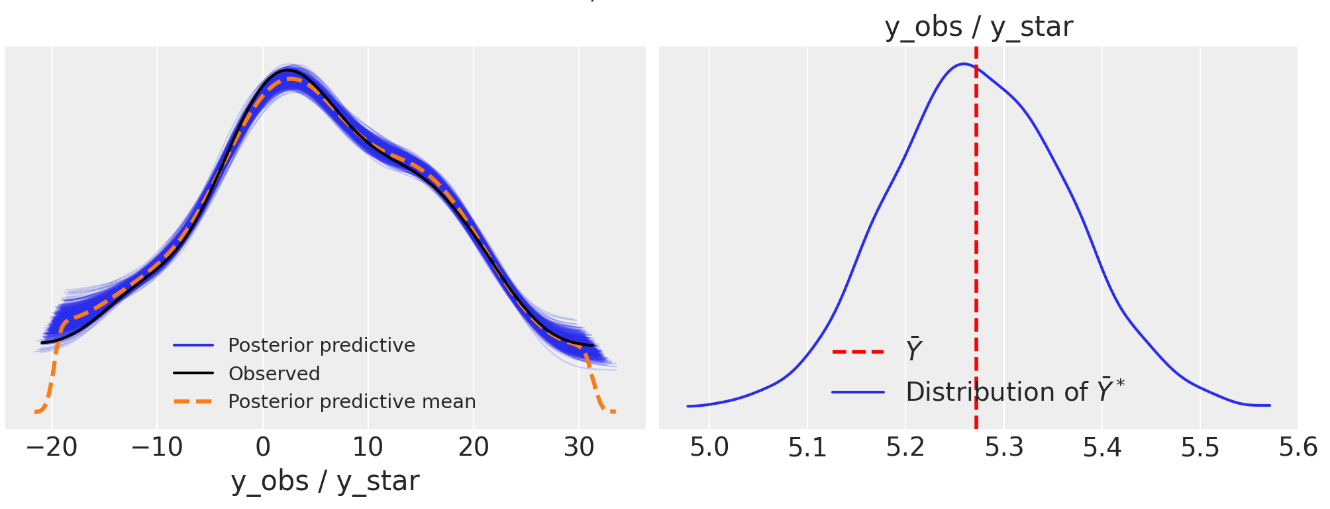
\includegraphics[width=0.95\textwidth]{img/ppc_lin}
  \caption{Posterior predictive graphical checks on a fitted model. On the left there is a comparison between the observed distribution of the response variable and the posterior predictive distribution of the generated samples, while the distribution of the average of the posterior predictive responses is depicted on the right.}\label{fig:ppc}
\end{figure}

\section{Experimental results}\label{sec:results}
\begin{comment}
  \begin{itemize}
    \item Comentar el método MCMC usado (\textit{emcee}) y por qué (vs. Metropolis u otros basados en gradiente como NUTS). Comentar que se lanzan varias cadenas en paralelo y luego se hace la media, para aumentar estabilidad.
    \item Comentar que se usa el MLE de los parámetros (perturbado) como punto de partida del algoritmo MCMC. Comentar la forma de estimación de MLE (varias iteraciones combinando una búsqueda global con una búsqueda local).
    \item Parámetros comunes de generación de datasets (granularidad de la malla, ...) y de la estrategia de ejecución (dónde se ejecuta, tiempos de ejecución, cuántas veces se repite para eliminar aleatoriedad, ...)
    \item Métricas usadas para medir el error.
    \item Contar los algoritmos de comparación usados.
    \item Mostrar tablas de resultados y gráficas.
\end{itemize}
\end{comment}

\subsection{Simulation studies}

\subsection{Application to real data}

\section{Conclusion}\label{sec:conclusion}

%%%%%%%%%%%%%%%%%%%%%%%%%%%%%%%%%%%%%%%%%%%%%%
%% Supplementary Material, if any, should   %%
%% be provided in {supplement} environment  %%
%% with title and short description.        %%
%%%%%%%%%%%%%%%%%%%%%%%%%%%%%%%%%%%%%%%%%%%%%%
\begin{supplement}
\stitle{Title of Supplement A}
\sdescription{Short description of Supplement A, with DOI and/or links to additional material (code, ...)}

\begin{comment}
  \begin{itemize}
  \item Detalles de la distribución log-posterior en cada caso?
  \item Comentar el uso de \(\log\sigma\) en lugar de \(\sigma^2\) para que el espacio de búsqueda sea no acotado.
  \item Comentar algunas decisiones de implementación: burn-in, thinning a la hora de hacer ppcs, ...
  \item Gráficos de las trazas, de algunas posterioris concretas, etc.
\end{itemize}
\end{comment}

\end{supplement}

\bibliographystyle{ba}
\bibliography{bibliography}

\begin{acks}[Acknowledgments]
This is an acknowledgements section.
\end{acks}


\end{document}
